En latch, eller flip-flop, er en 1bit minne.
Den kan lagre en enkel tilstand, av eller på.
Et større minne settes sammen av flere flip-flops.



\paragraph{SR-latch} \mbox{} \\
Den enkleste latchen består av to input og to output.
\begin{figure}[H]
  \caption{SR-latch med set og release.}
  \centering
  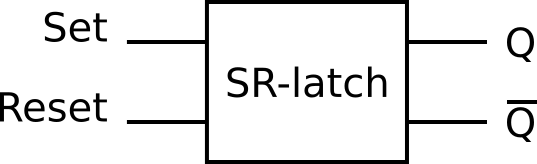
\includegraphics[width=0.5\textwidth]{./img/sr-latch}
\end{figure}
Når set aktiveres skifter latchen tilstand til 1 og når reset aktiveres
skifter den tilstand til 0.
Når verken er aktivert beholder den sin tilstand.



\paragraph{$\overline{SR}$-latch} \mbox{} \\
En implementasjon av sr-latchen kan bygges av to NAND-porter.
\emph{Merk at input er not S og not R, altså inverterte av S og R.}
\begin{figure}[H]
  \centering
  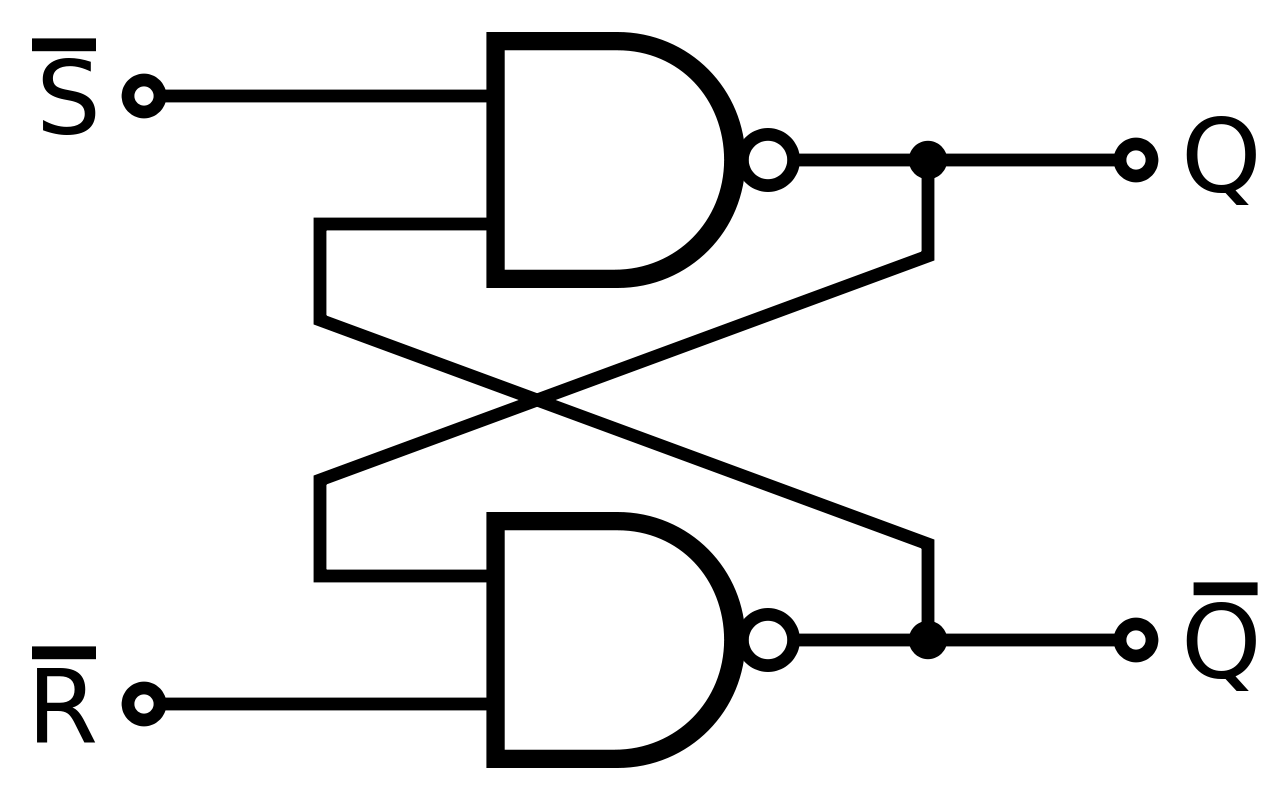
\includegraphics[width=0.5\textwidth]{./img/not-sr}
\end{figure}
Husk at input er not S og derfor er 0 aktivert og 1 deaktivert på inngangen.
\begin{table}[H]
  \centering
  \begin{tabular}{c|c|c|c}
    $\overline{S}$ & $\overline{R}$ & Q & $\overline{Q}$ \\ \hline
    1 & 0 & 0 & 1 \\
    1 & 1 & 0 & 1 \\
    0 & 1 & 1 & 0 \\
    1 & 1 & 1 & 0 \\
    0 & 0 & 1 & 1
  \end{tabular}
\end{table}
Tenk igjennom logikken og se til at du forstår det (eller for å se om jeg har
skrevet feil).



\paragraph{Synkron SR-latch} \mbox{} \\
Vi kan kontrollere en latch så den kun skifter tilstand når den mottar
et klokkesignal.
Dette brukes for å synkronisere kretser og registere.
\begin{figure}[H]
  \caption{Klokkestyrt latch laget av AND og NOR.}
  \centering
  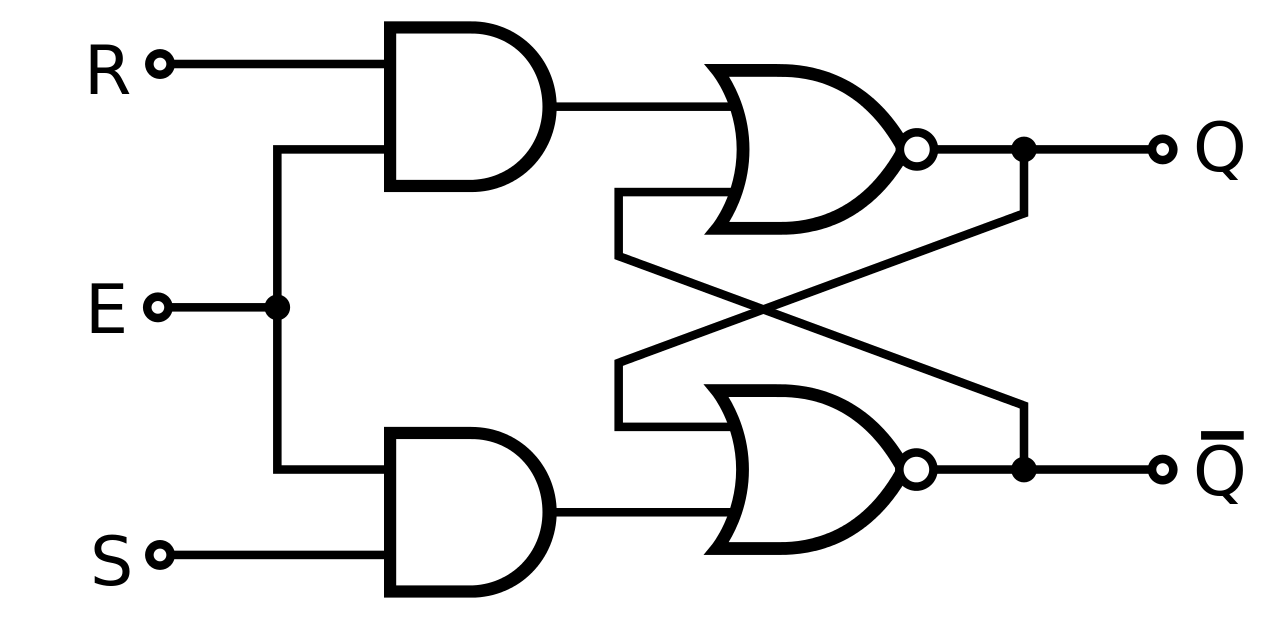
\includegraphics[width=0.67\textwidth]{./img/klokket-sr}
\end{figure}



\paragraph{D-latch} \mbox{} \\
En d-latch kan anses som en én-input sr-latch.
Denne forhindrer bruk av ulovlige inputkombinasjoner.
\begin{figure}[H]
  \caption{d-latch}
  \centering
  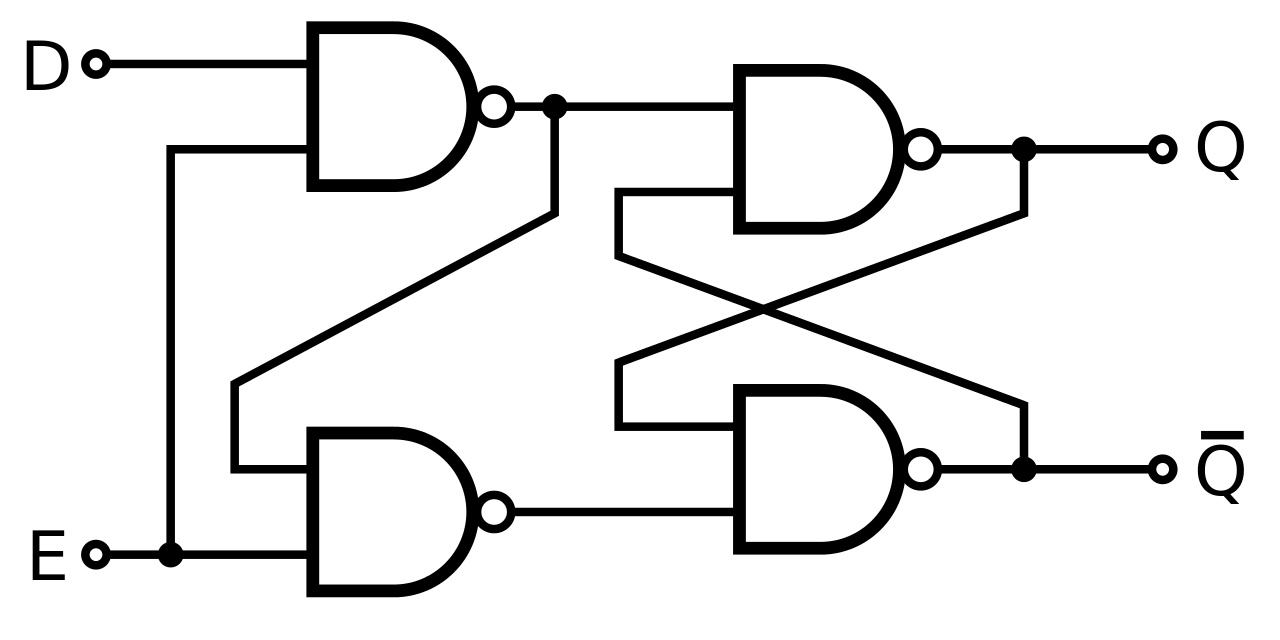
\includegraphics[width=0.67\textwidth]{./img/klokket-dlatch}
\end{figure}
